% shall we have a discussion section after methods and results?
% Discussion
% 	- possibility of using the "domination graph" as data,
% 	where decks are nodes and win rates are the directed
% 	edges
% 	- there is some correlation in the win rate dictionary
% 	distribution, as cards appear alongside other cards
% 	- we don't use a Hessian or Jacobian based opt method,
% 	which would have been useful to understand sensitivity

\subsection{Playtesting simulator}

To serve as a data source for quantitative analysis, we create
a playtesting simulator of a simplified auto battler game. 
This simulator is designed for research. It allows the user to 
create cards with new mechanics and run tournaments between
arbitrary decks. 

\subsubsection{Simplified game definition} \label{sec:ab-game-def}

Cards have nonnegative integer statistics including health points, 
attack, and parameters pertaining to a special mechanism. Such special parameters
developed include the following:

% consider table instead of bullets for space
\begin{itemize}
	\item Explosion damage. When the card dies, it damages
	each of the opponent's cards by this many health points.
	\item Heal amount. Prior to entering combat, the card 
	restores this many health points to its player's rightmost
	card
	\item Attack growth per hit. When the card takes damage, its
	attack increases by this many points.
	\item Explosion heal. When the card dies, it heals
	each of its player's other cards by this many health points.
	\item Heal donation percent. When the card would be healed,
	it instead restores this many percent of the health points
	to itself and donates the remaining health points to its
	player's other cards evenly.
	\item Armor points. The card starts with this many armor points.
	When the card would be damaged, it instead loses an armor point.
	When the card has zero armor points, it may be damaged normally.
	\item Damage split percent. When the card would be damaged,
	it instead receives this many percent of the damage to itself
	and splits the remaining damage evenly to its player's other cards.
	\item Middle age. Prior to entering combat, the card increases its
	attack by 1 if it has not participated in this many combat phases.
	After this many combat phases, the card decreases its attack by 1
	before entering combat.
	\item Target age. When the card dies, if it participated in this many
	combat phases, deal this many damage points to each of the opponent's
	cards. If the card participated in fewer than this many combat phases, 
	heal each of its player's other cards by health points equal to the
	number of combat phases in which the card participated.
	\item Detonation time. When the card has been healed or damaged this
	many times, the card and its opponent both die.
\end{itemize}

Other card mechanics without parameters include the ability to copy the 
attack of the opponent's cards (morphing enemies) and the ability to swap 
its health points and attack whenever its attack is greater than its health 
points (survivalist).

\subsubsection{Automated playtesting procedure} \label{sec:tourney}

For the simulator, gameplay proceeds as follows:

\begin{enumerate}
	\item Each player in a tournament selects an ordered list
	of cards to be their deck.
	\item Prior to combat, the deck is arranged left-to-right.
	\item Each combat phase pits the leftmost surviving card
	of each player against each other. The cards take damage by 
	reducing their health points by their opponent card's attack.
	Cards with zero or fewer health points are dead. Surviving cards
	are arranged to be the rightmost card of their respective decks.
	\item Repeat combat until one or fewer players has a surviving card
	or the maximum number of combat phases allowed has been reached.
	If both or neither players a surviving card, the game is a tie.
	Otherwise, the player with a surviving card wins.
	\item Proceed with the tournament in a round-robin fashion. Each 
	player plays a game with each other player once.
\end{enumerate}

Combined with a metric measuring the health of the metagame, this simulator 
forms an approximation algorithm that estimates parity within the game.

\subsection{Metrics} \label{sec:metrics}

Quantitative measures of metagame health are needed to guide 
card statistic optimization. We present metrics built upon the
output data of the playtesting simulator described previously.

The playtesting simulation outputs a data vector $v$.
Each entry $v_i \in [-1, 1]$ represents the average payoff of
the deck at index $i$ during the last round of playtesting in
the optimization process. A payoff of 1 indicates a win. A
payoff of 0 means a tie, and a loss results in a payoff of -1.
The average of these payoffs over the course of the simulated
tournament for a deck make up the entries of $v$.

We then transform $v$ into another vector of length $n$ which maps a card to the
average win rate of the decks in which the card appears. This
vector $w$ has entries
$w_j \in [0, 1]$, the average win rate of the decks in which
the card at index $j$ appears. We present three metrics that 
use this distribution of win rates among the cards.

% run Jack's `plot.py` script

% \subsubsection{Per-card payoff}

% \begin{equation}
% 	\mathrm{PCP} = \frac{1}{n} \sum_j \left|\mathrm{payoff}(w_j)\right|^2
% \end{equation}

\subsubsection{Standard deviation metric}

\begin{equation}
	\mathrm{SDM} = \sqrt{\frac{1}{n} \sum_j \left|w_j - \left(\frac{1}{n}\sum_j w_j\right)\right|^2}
\end{equation}

Standard deviation of the win rates is a metric we may seek to minimize. Doing so may avoid cards with
very high or low win rates compared to others.

\subsubsection{Entropy metric}

\begin{equation}
	\mathrm{EM} = -\sum_j \frac{w_j}{\sum_j w_j} \log\left(\frac{w_j}{\sum_j w_j}\right)
\end{equation}

Entropy of the win rates is a metric we may seek to maximize. When entropy is maximized, we approach a uniform
distribution of cards over win rates.

\subsubsection{Other metrics}

Our framework is flexible; researchers and designers alike may develop their own metrics corresponding to their
own ideas of what constitutes a healthy metagame. For example, a game designer may know from historical data that
a certain distribution of cards or decks over win rates corresponded to a period of celebrated parity in the metagame. 
The designer could conceivably use the Wasserstein distance or Kullback--Leibler 
divergence between this historical distribution and another distribution as a metric. Minimizing this metric 
might maintain similar levels of parity through future iterations of card releases.

\subsection{Optimization}

We use the \citeauthor{gad2021pygad}'s \shortcite{gad2021pygad} PyGAD python library for genetic optimization algorithms. This will attempt to find the optimal values of
parameters, which may include health points, attack, and special parameters, that optimizes
the chosen metric.

We constrain the genetic algorithm to consider integer values of the parameters between 1 and 10, inclusive. While hyperparameter tuning may have yielded better results,
we chose to run the genetic algorithm with 8 solutions and 4 parents mating per population for 32 generations in each experiment.

\subsection{Qualitative analysis}

Another way of understanding the landscape of the metagame is through more qualitative methods. We look at two different ways of plotting data about the game results which give insights into the health and stability of the metagame. 

The first plot is a sweep over two variables, typically of the same card, although not necessarily. This gives a visual representation of the metagame throughout various configurations, and can lead to some interesting insights about the relationship between cards.

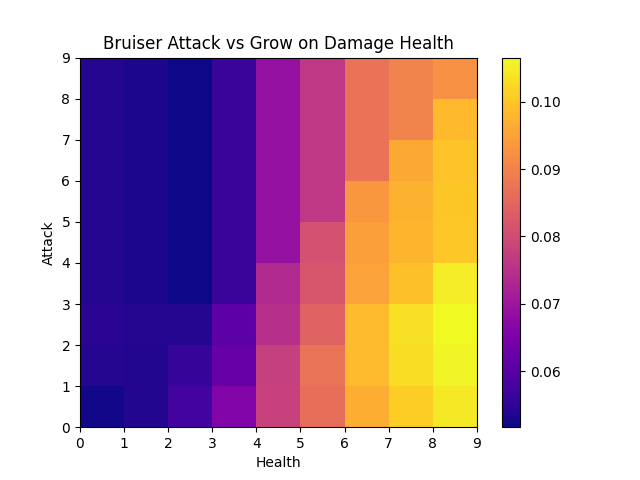
\includegraphics[width=10cm, height=8cm]{bruiser_vs_grow} \label{fig:bruiser_vs_grow}

Take, for example, the plot in Figure~\ref{fig:bruiser_vs_grow}, of the value of the standard deviation metric given various values for the attack of the bruiser card and the health of the grow on damage card. The bruiser card is a vanilla card with a high attack (although variable in this situation) and one health point. The grow on damage card has a mechanic where each time it takes damage it gains one attack. Initially this card has no attack, and in this situation has a variable amount of health. 

In the figure we can see that configurations in the upper left corner, where the attack of the bruiser is greater than the health of the grow on damage card, tend to be much more favorable than the configurations in the lower right corner, where the opposite is true. This evidence supports the intuitive idea that the bruiser's high attack is a good counter to the grow on damage card, because it can quickly remove the monster before it has had enough interactions to grow its damage to a large number. This kind of information can be quite useful to a game designer, who can see very clearly that the inclusion of a high damage card can improve the metagame dramatically if the grow on damage card is found to be too powerful.


\subsection{Experiment design}

% in methods: only describe the phases of experiments in a high level -- 1. build decks 2. tournaments 3. ... their common pattern
% describe set up, techniques; write about analysis and numbers in results

Our experiments share common phases.

\begin{enumerate}
	\item Build decks. We generate a set of cards and their associated attack, health points, and special parameters.
	Depending on the experiment, some or all of these variables may be varied from simulation to simulation during the optimization process.
	From this set of cards, the decks are permutations of 3 cards from the set, allowing for duplicates.
	\item Run tournaments. We pit the decks against each other in a round-robin tournament. For $n$ decks,
	the number of matches is $n(n-1)/2 = O(n^2)$. A complete round-robin tournament quickly becomes prohibitively large to simulate.
	Thus, we may want to sample from every possible matchup in order to estimate the win rates of cards and decks. We do this by 
	partitioning the decks into groups of uniform size and running round-robin tournaments within these groups.
	\item Optimize. These tournaments are run within each iteration of our genetic algorithm to produce a metric estimating the best
	possible health of the metagame with respect to parameters of the built decks.
\end{enumerate}
